\let\negmedspace\undefined
\let\negthickspace\undefined
\documentclass[journal]{IEEEtran}
\usepackage[a5paper, margin=10mm, onecolumn]{geometry}
%\usepackage{lmodern} % Ensure lmodern is loaded for pdflatex
\usepackage{tfrupee} % Include tfrupee package

\setlength{\headheight}{1cm} % Set the height of the header box
\setlength{\headsep}{0mm}     % Set the distance between the header box and the top of the text

\usepackage{gvv-book}
\usepackage{comment}
\usepackage{gvv}
\usepackage{cite}
\usepackage{amsmath,amssymb,amsfonts,amsthm}
\usepackage{algorithmic}
\usepackage{graphicx}
\usepackage{textcomp}
\usepackage{xcolor}
%\usepackage{txfonts}
\usepackage{listings}
\usepackage{enumitem}
\usepackage{mathtools}
\usepackage{gensymb}
\usepackage{comment}
\usepackage[breaklinks=true]{hyperref}
\usepackage{tkz-euclide} 
\usepackage{listings}
% \usepackage{gvv}                                        
\def\inputGnumericTable{}                                 
\usepackage[latin1]{inputenc}                                
\usepackage{color}                                            
\usepackage{array}                                            
\usepackage{longtable}                                       
\usepackage{calc}                                             
\usepackage{multirow}                                         
\usepackage{hhline}                                           
\usepackage{ifthen}                                           
\usepackage{lscape}
\usepackage{circuitikz}
\tikzstyle{block} = [rectangle, draw, fill=blue!20, 
    text width=4em, text centered, rounded corners, minimum height=3em]
\tikzstyle{sum} = [draw, fill=blue!10, circle, minimum size=1cm, node distance=1.5cm]
\tikzstyle{input} = [coordinate]
\tikzstyle{output} = [coordinate]


\begin{document}

\bibliographystyle{IEEEtran}
\vspace{3cm}

\title{12.547}
\author{EE25BTECH11013 - Bhargav}
\maketitle
    {\let\newpage\relax\maketitle}

\renewcommand{\thefigure}{\theenumi}
\renewcommand{\thetable}{\theenumi}
\setlength{\intextsep}{10pt} % Space between text and floats

\numberwithin{equation}{enumi}
\numberwithin{figure}{enumi}
\renewcommand{\thetable}{\theenumi}

\textbf{Question}: \\
Consider $\mathbf{R^3}$ with the usual inner product. If d  is the distance from (1,1,1) to the subspace span $\cbrak{(1,1,0), (0,1,1)}$ of $\mathbf{R^3}$, then $3d^2$ is

\solution \\
Let
$\vec{W} = \operatorname{span}\cbrak{u_1, u_2}$\\
Where $\vec{U} = \myvec{u_1 & u_2}$ \\

The distance from $\vec{P} = \myvec{1 \\ 1 \\ 1}$ to the subspace span $\vec{W}$ can be found by finding the projection of $\vec{P}$ onto $\vec{W}$.\\

 Let $\vec{U}\vec{x}$ be the projection of $\vec{P}$ on the span $\vec{W}$, where $\vec{x} \in \mathbf{R}^3$

\begin{align}
\vec{U^T}\brak{\vec{P-Ux}}=0
\end{align}
(since $\vec{U}$ is perpendicular to $\vec{P-Ux}$)
\begin{align}
\implies \vec{U^T}\vec{U}\vec{x} = \vec{U^T}\vec{P}
\end{align}
Since the columns of $\vec{U}$ are Linearly independent, so are the columns of $\vec{U^T}\vec{U}$ and hence $\vec{U^T}\vec{U}$ is invertible 
\begin{align}
\vec{x} = \brak{\vec{U^T}\vec{U}}^{-1} \vec{U^T}\vec{P}
\end{align}
Hence the projection of $\vec{P}$ on the span $\vec{W}$ is
\begin{align}
\vec{U}\vec{x} = \vec{U}\brak{\vec{U^T}\vec{U}}^{-1} \vec{U^T}\vec{P}
\end{align}

The distance of $\vec{P}$ from the span $\vec{W}$ is:
\begin{align}
d = \norm{\vec{P} - \vec{U}\vec{x}}
\end{align}
\begin{align}
d = \norm{\vec{P} - \vec{U}\brak{\vec{U^T}\vec{U}}^{-1} \vec{U^T}\vec{P}}
\end{align}
\begin{align}
\vec{P} = \myvec{1 \\ 1 \\ 1}, \vec{U} = \myvec{1 & 0 \\ 1 & 1 \\ 0 & 1}
\end{align}
Substituting the values in \brak{0.6}:
\begin{align}
d = \frac{1}{\sqrt{3}}
\end{align}


\boxed{3d^2 = 1}

    \begin{figure}[H]
        \centering
        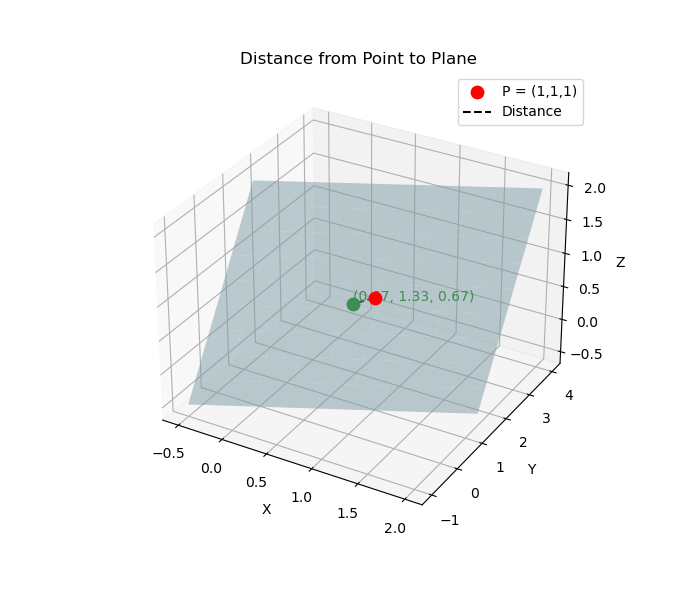
\includegraphics[height=0.5\textheight, keepaspectratio]{figs/Figure_1.png}
        \label{figure_1}
    \end{figure}

\end{document}
